\documentclass[11pt,]{article}
\usepackage[left=1in,top=1in,right=1in,bottom=1in]{geometry}
\newcommand*{\authorfont}{\fontfamily{phv}\selectfont}
\usepackage[]{mathpazo}


  \usepackage[T1]{fontenc}
  \usepackage[utf8]{inputenc}




\usepackage{abstract}
\renewcommand{\abstractname}{}    % clear the title
\renewcommand{\absnamepos}{empty} % originally center

\renewenvironment{abstract}
 {{%
    \setlength{\leftmargin}{0mm}
    \setlength{\rightmargin}{\leftmargin}%
  }%
  \relax}
 {\endlist}

\makeatletter
\def\@maketitle{%
  \newpage
%  \null
%  \vskip 2em%
%  \begin{center}%
  \let \footnote \thanks
    {\fontsize{18}{20}\selectfont\raggedright  \setlength{\parindent}{0pt} \@title \par}%
}
%\fi
\makeatother




\setcounter{secnumdepth}{0}


\usepackage{graphicx,grffile}
\makeatletter
\def\maxwidth{\ifdim\Gin@nat@width>\linewidth\linewidth\else\Gin@nat@width\fi}
\def\maxheight{\ifdim\Gin@nat@height>\textheight\textheight\else\Gin@nat@height\fi}
\makeatother
% Scale images if necessary, so that they will not overflow the page
% margins by default, and it is still possible to overwrite the defaults
% using explicit options in \includegraphics[width, height, ...]{}
\setkeys{Gin}{width=\maxwidth,height=\maxheight,keepaspectratio}


\title{Application of Machine Learning on Fundamental Stock Price Analysis  }



\author{\Large Albina Cako, BSc\vspace{0.05in} \newline\normalsize\emph{York University, Certificate in Machine Learning}   \and \Large Colin Green, BSc\vspace{0.05in} \newline\normalsize\emph{York University, Certificate in Machine Learning}   \and \Large Lucy Zhang, BSc\vspace{0.05in} \newline\normalsize\emph{York University, Certificate in Machine Learning}   \and \Large Sean X. Zhang, MSc\vspace{0.05in} \newline\normalsize\emph{York University, Certificate in Machine Learning}  }


\date{}

\usepackage{titlesec}

\titleformat*{\section}{\normalsize\bfseries}
\titleformat*{\subsection}{\normalsize\itshape}
\titleformat*{\subsubsection}{\normalsize\itshape}
\titleformat*{\paragraph}{\normalsize\itshape}
\titleformat*{\subparagraph}{\normalsize\itshape}





\newtheorem{hypothesis}{Hypothesis}
\usepackage{setspace}


% set default figure placement to htbp
\makeatletter
\def\fps@figure{htbp}
\makeatother

\usepackage{hyperref}
\usepackage{graphicx}
\usepackage{subfig}

% move the hyperref stuff down here, after header-includes, to allow for - \usepackage{hyperref}

\makeatletter
\@ifpackageloaded{hyperref}{}{%
\ifxetex
  \PassOptionsToPackage{hyphens}{url}\usepackage[setpagesize=false, % page size defined by xetex
              unicode=false, % unicode breaks when used with xetex
              xetex]{hyperref}
\else
  \PassOptionsToPackage{hyphens}{url}\usepackage[draft,unicode=true]{hyperref}
\fi
}

\@ifpackageloaded{color}{
    \PassOptionsToPackage{usenames,dvipsnames}{color}
}{%
    \usepackage[usenames,dvipsnames]{color}
}
\makeatother
\hypersetup{breaklinks=true,
            bookmarks=true,
            pdfauthor={Albina Cako, BSc (York University, Certificate in Machine Learning) and Colin Green, BSc (York University, Certificate in Machine Learning) and Lucy Zhang, BSc (York University, Certificate in Machine Learning) and Sean X. Zhang, MSc (York University, Certificate in Machine Learning)},
             pdfkeywords = {stock price, fundamental analysis, machine learning, R},  
            pdftitle={Application of Machine Learning on Fundamental Stock Price Analysis},
            colorlinks=true,
            citecolor=blue,
            urlcolor=blue,
            linkcolor=magenta,
            pdfborder={0 0 0}}
\urlstyle{same}  % don't use monospace font for urls

% Add an option for endnotes. -----


% add tightlist ----------
\providecommand{\tightlist}{%
\setlength{\itemsep}{0pt}\setlength{\parskip}{0pt}}

% add some other packages ----------

% \usepackage{multicol}
% This should regulate where figures float
% See: https://tex.stackexchange.com/questions/2275/keeping-tables-figures-close-to-where-they-are-mentioned
\usepackage[section]{placeins}


\begin{document}
	
% \pagenumbering{arabic}% resets `page` counter to 1 
%
% \maketitle

{% \usefont{T1}{pnc}{m}{n}
\setlength{\parindent}{0pt}
\thispagestyle{plain}
{\fontsize{18}{20}\selectfont\raggedright 
\maketitle  % title \par  

}

{
   \vskip 13.5pt\relax \normalsize\fontsize{11}{12} 
\textbf{\authorfont Albina Cako, BSc} \hskip 15pt \emph{\small York University, Certificate in Machine Learning}   \par \textbf{\authorfont Colin Green, BSc} \hskip 15pt \emph{\small York University, Certificate in Machine Learning}   \par \textbf{\authorfont Lucy Zhang, BSc} \hskip 15pt \emph{\small York University, Certificate in Machine Learning}   \par \textbf{\authorfont Sean X. Zhang, MSc} \hskip 15pt \emph{\small York University, Certificate in Machine Learning}   

}

}








\begin{abstract}

    \hbox{\vrule height .2pt width 39.14pc}

    \vskip 8.5pt % \small 

\noindent Abstract:


\vskip 8.5pt \noindent \emph{Keywords}: stock price, fundamental analysis, machine learning, R \par

    \hbox{\vrule height .2pt width 39.14pc}



\end{abstract}


\vskip -8.5pt


 % removetitleabstract

\noindent  

\hypertarget{introduction}{%
\section{Introduction}\label{introduction}}

\hypertarget{methodology}{%
\section{Methodology}\label{methodology}}

\hypertarget{data-preprocessing}{%
\subsection{Data Preprocessing}\label{data-preprocessing}}

\hypertarget{missing-values}{%
\subsection{Missing Values}\label{missing-values}}

\hypertarget{outliers}{%
\subsection{Outliers}\label{outliers}}

\hypertarget{data-curation}{%
\subsection{Data Curation}\label{data-curation}}

\hypertarget{modeling}{%
\subsection{Modeling}\label{modeling}}

\hypertarget{deployment}{%
\subsection{Deployment}\label{deployment}}

\hypertarget{results}{%
\section{Results}\label{results}}

\hypertarget{data-exploration}{%
\subsection{Data Exploration}\label{data-exploration}}

\hypertarget{principle-component-analysis}{%
\subsection{Principle Component
Analysis}\label{principle-component-analysis}}

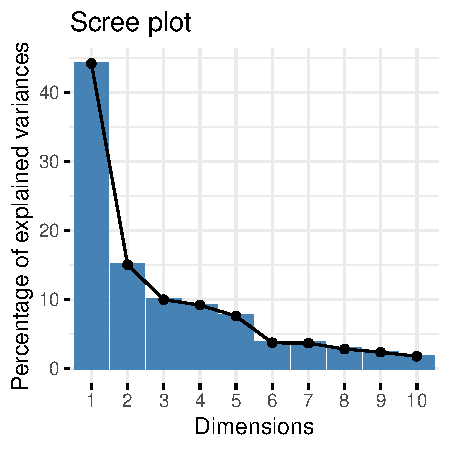
\includegraphics{stock_analysis_files/figure-latex/scree-1.pdf}
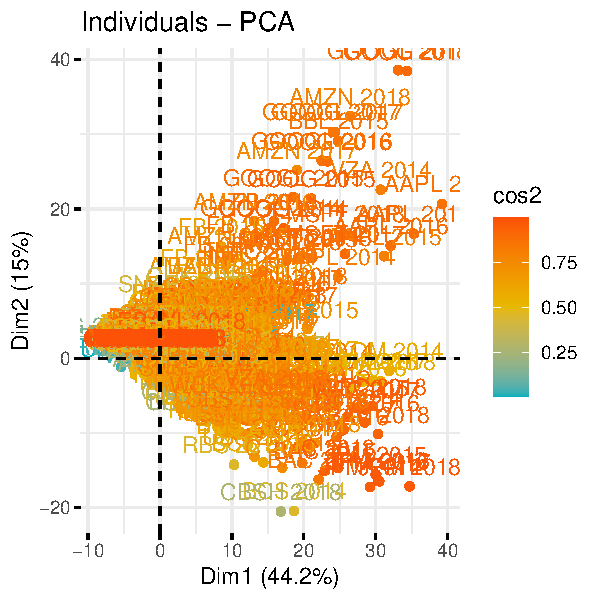
\includegraphics{stock_analysis_files/figure-latex/PCAind-1.pdf}
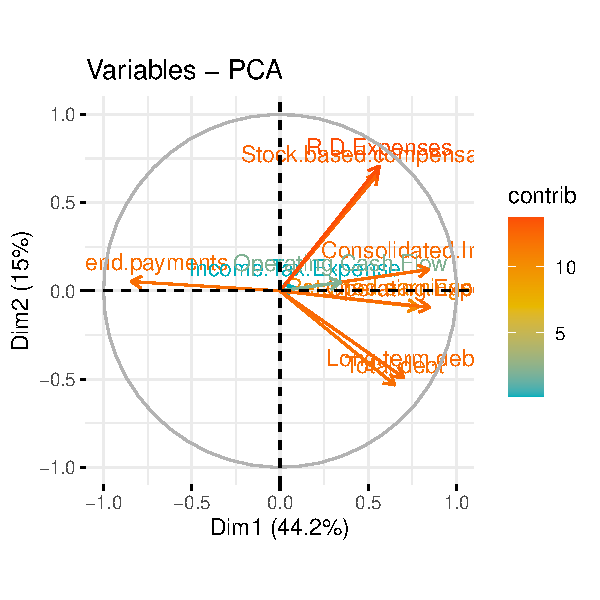
\includegraphics{stock_analysis_files/figure-latex/PCAvar-1.pdf}

\hypertarget{k-means-clustering}{%
\subsection{K Means Clustering}\label{k-means-clustering}}

\begin{figure}
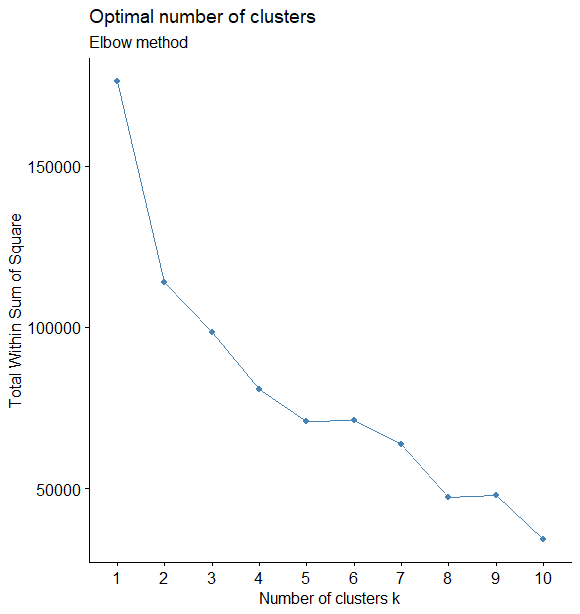
\includegraphics[width=1\linewidth,height=0.7\textheight]{unsupervised_elbow} \caption{Elbow method}\label{fig:elbow}
\end{figure}

\begin{figure}
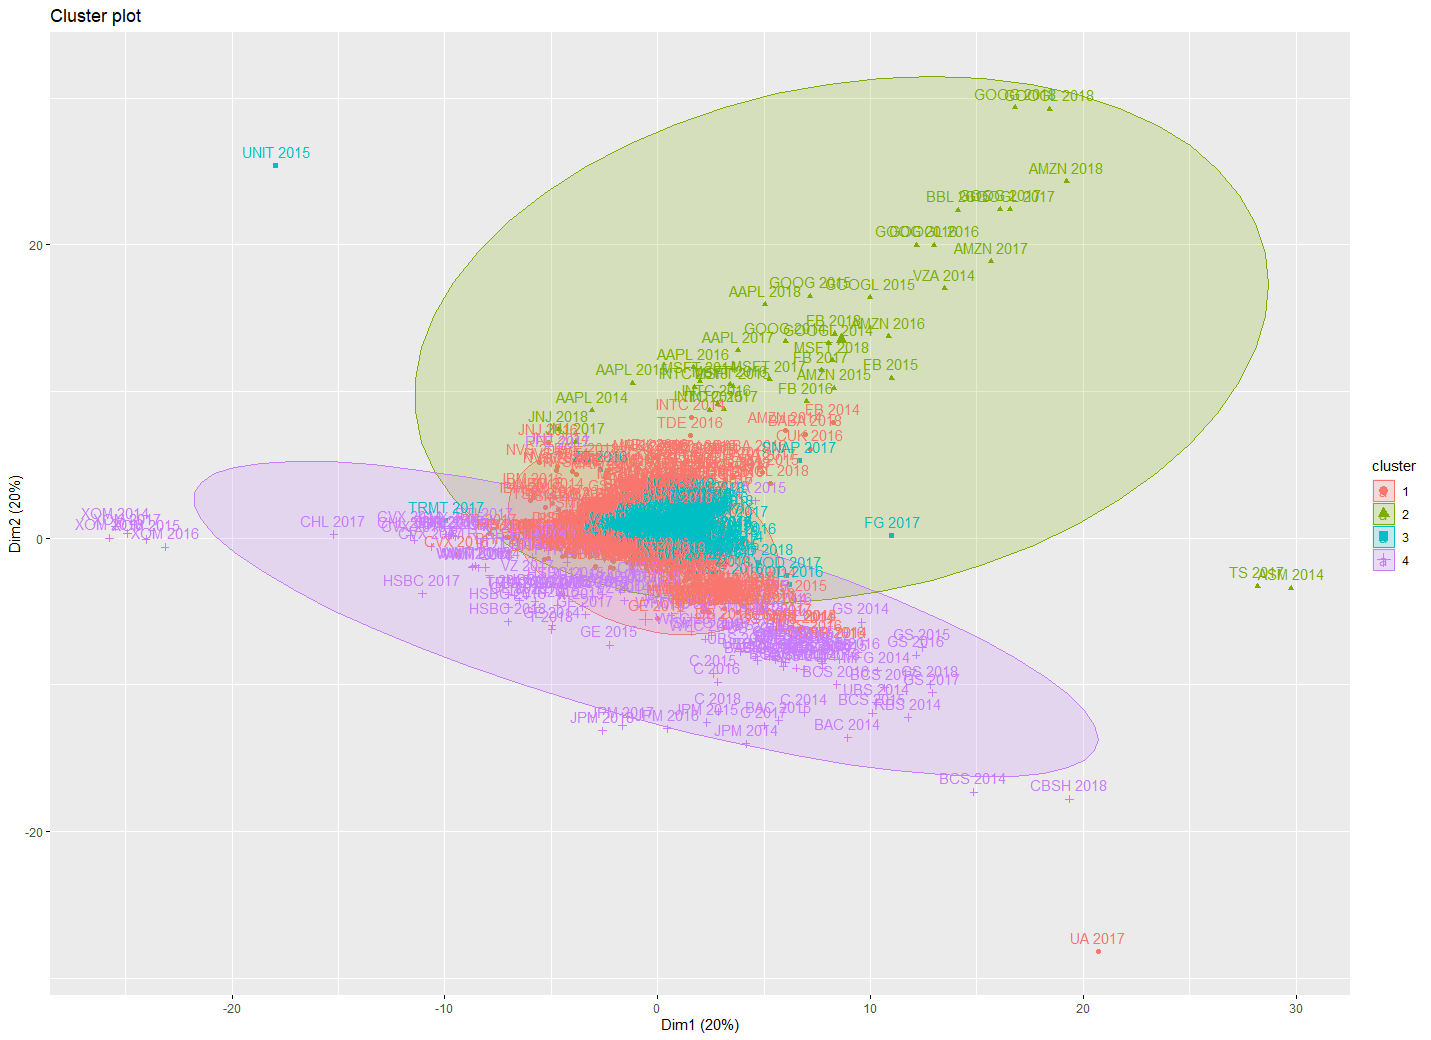
\includegraphics[width=1\linewidth,height=0.7\textheight]{cluster_image} \caption{K means clustering, k = 4}\label{fig:cluster}
\end{figure}

\hypertarget{modeling-1}{%
\subsection{Modeling}\label{modeling-1}}

\#\#\#Random Forest \#\#\#XGBoost \#\#\#Lasso Regression \#\#\#GBM
\#\#\#Model Selection

\hypertarget{discussion}{%
\section{Discussion}\label{discussion}}





\newpage
\singlespacing 
\end{document}
